%!TEX root = lec16.tex
% ================================================================================
% Lecture 16 — Slide 39
% ================================================================================
\begin{frame}[t]
\mytitle{Slide 39: Rebuild Services --- Analyze Work, Find Waste, Build Tools}

\begin{columns}[T,totalwidth=\textwidth]

% ------------------------------------------------------------
\begin{column}[T]{0.50\textwidth}
\footnotesize
\vspace{-2mm}

\textbf{Step 1: Look at our daily workflow}
\begin{itemize}
  \item Where do we \rtext{repeat} the same steps?
  \item Where do we \rtext{copy/paste} between systems?
  \item Where do we \rtext{wait} for data, plots, approvals?
  \item Where do we \rtext{lose context} (emails, chats, files)?
\end{itemize}

\vspace{2mm}
\textbf{Step 2: Turn waste into tools}
\begin{itemize}
  \item define a clear \y{input/output interface}
  \item make it callable (API / function / agent tool)
  \item reuse it everywhere: DAWID, scripts, services, pipelines
\end{itemize}

\end{column}

% ------------------------------------------------------------
\begin{column}[T]{0.50\textwidth}
\vspace{-2mm}

\begin{center}
\scalebox{0.6}{
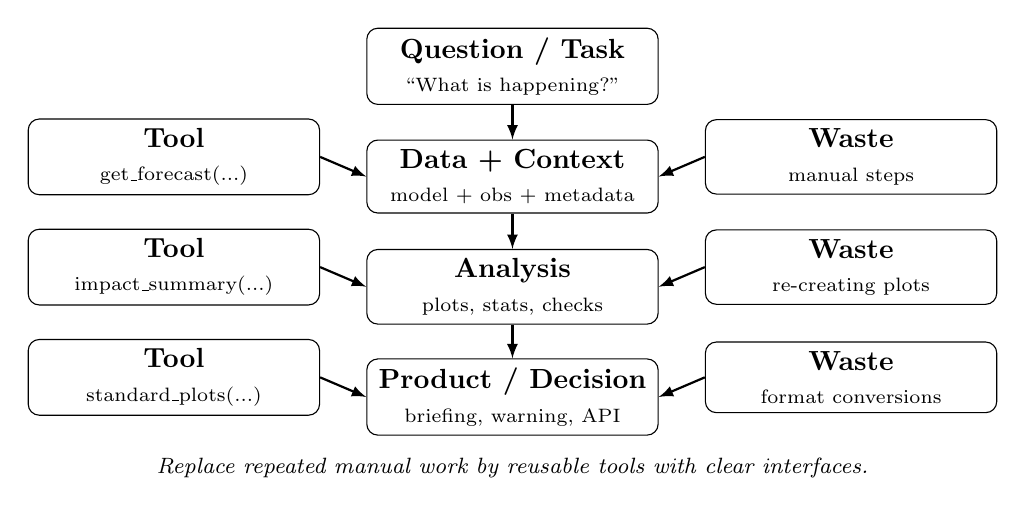
\begin{tikzpicture}[x=1cm,y=1cm,>=latex]

\tikzstyle{box}=[draw,rounded corners,align=center,minimum width=3.7cm,minimum height=0.85cm]
\tikzstyle{waste}=[draw,rounded corners,align=center,minimum width=3.7cm,minimum height=0.75cm]
\tikzstyle{tool}=[draw,rounded corners,align=center,minimum width=3.7cm,minimum height=0.75cm]
\tikzstyle{arrow}=[->,thick]

% ------------------------------------------------------------
% main chain (more vertical spacing)
% ------------------------------------------------------------
\node[box] (q) at (0,4.2) {\textbf{Question / Task}\\{\scriptsize ``What is happening?''}};
\node[box] (d) at (0,2.8) {\textbf{Data + Context}\\{\scriptsize model + obs + metadata}};
\node[box] (a) at (0,1.4) {\textbf{Analysis}\\{\scriptsize plots, stats, checks}};
\node[box] (p) at (0,0.0) {\textbf{Product / Decision}\\{\scriptsize briefing, warning, API}};

\draw[arrow] (q) -- (d);
\draw[arrow] (d) -- (a);
\draw[arrow] (a) -- (p);

% ------------------------------------------------------------
% waste tags on the right (aligned to chain)
% ------------------------------------------------------------
\node[waste] (w1) at (4.3,3.05) {\rtext{\textbf{Waste}}\\{\scriptsize manual steps}};
\node[waste] (w2) at (4.3,1.65) {\rtext{\textbf{Waste}}\\{\scriptsize re-creating plots}};
\node[waste] (w3) at (4.3,0.25) {\rtext{\textbf{Waste}}\\{\scriptsize format conversions}};

\draw[arrow] (w1.west) -- (d.east);
\draw[arrow] (w2.west) -- (a.east);
\draw[arrow] (w3.west) -- (p.east);

% ------------------------------------------------------------
% tools on the left (aligned to chain)
% ------------------------------------------------------------
\node[tool] (t1) at (-4.3,3.05) {\y{\textbf{Tool}}\\{\scriptsize get\_forecast(...)}};
\node[tool] (t2) at (-4.3,1.65) {\y{\textbf{Tool}}\\{\scriptsize impact\_summary(...)}};
\node[tool] (t3) at (-4.3,0.25) {\y{\textbf{Tool}}\\{\scriptsize standard\_plots(...)}};

\draw[arrow] (t1.east) -- (d.west);
\draw[arrow] (t2.east) -- (a.west);
\draw[arrow] (t3.east) -- (p.west);

% ------------------------------------------------------------
% small caption
% ------------------------------------------------------------
\node[align=center] at (0,-0.9) {\footnotesize \textit{Replace repeated manual work by reusable tools with clear interfaces.}};

\end{tikzpicture}
}
\end{center}

\end{column}

\end{columns}

\vspace{2mm}
\rtext{\textbf{Key message:}}
If a task repeats, it should become a \y{tool}.

\end{frame}
